\setlength{\columnsep}{3pt}
\begin{flushleft}
	
	\paragraph{}
	\bigskip
	
	\begin{figure}[h!]
		\centering
		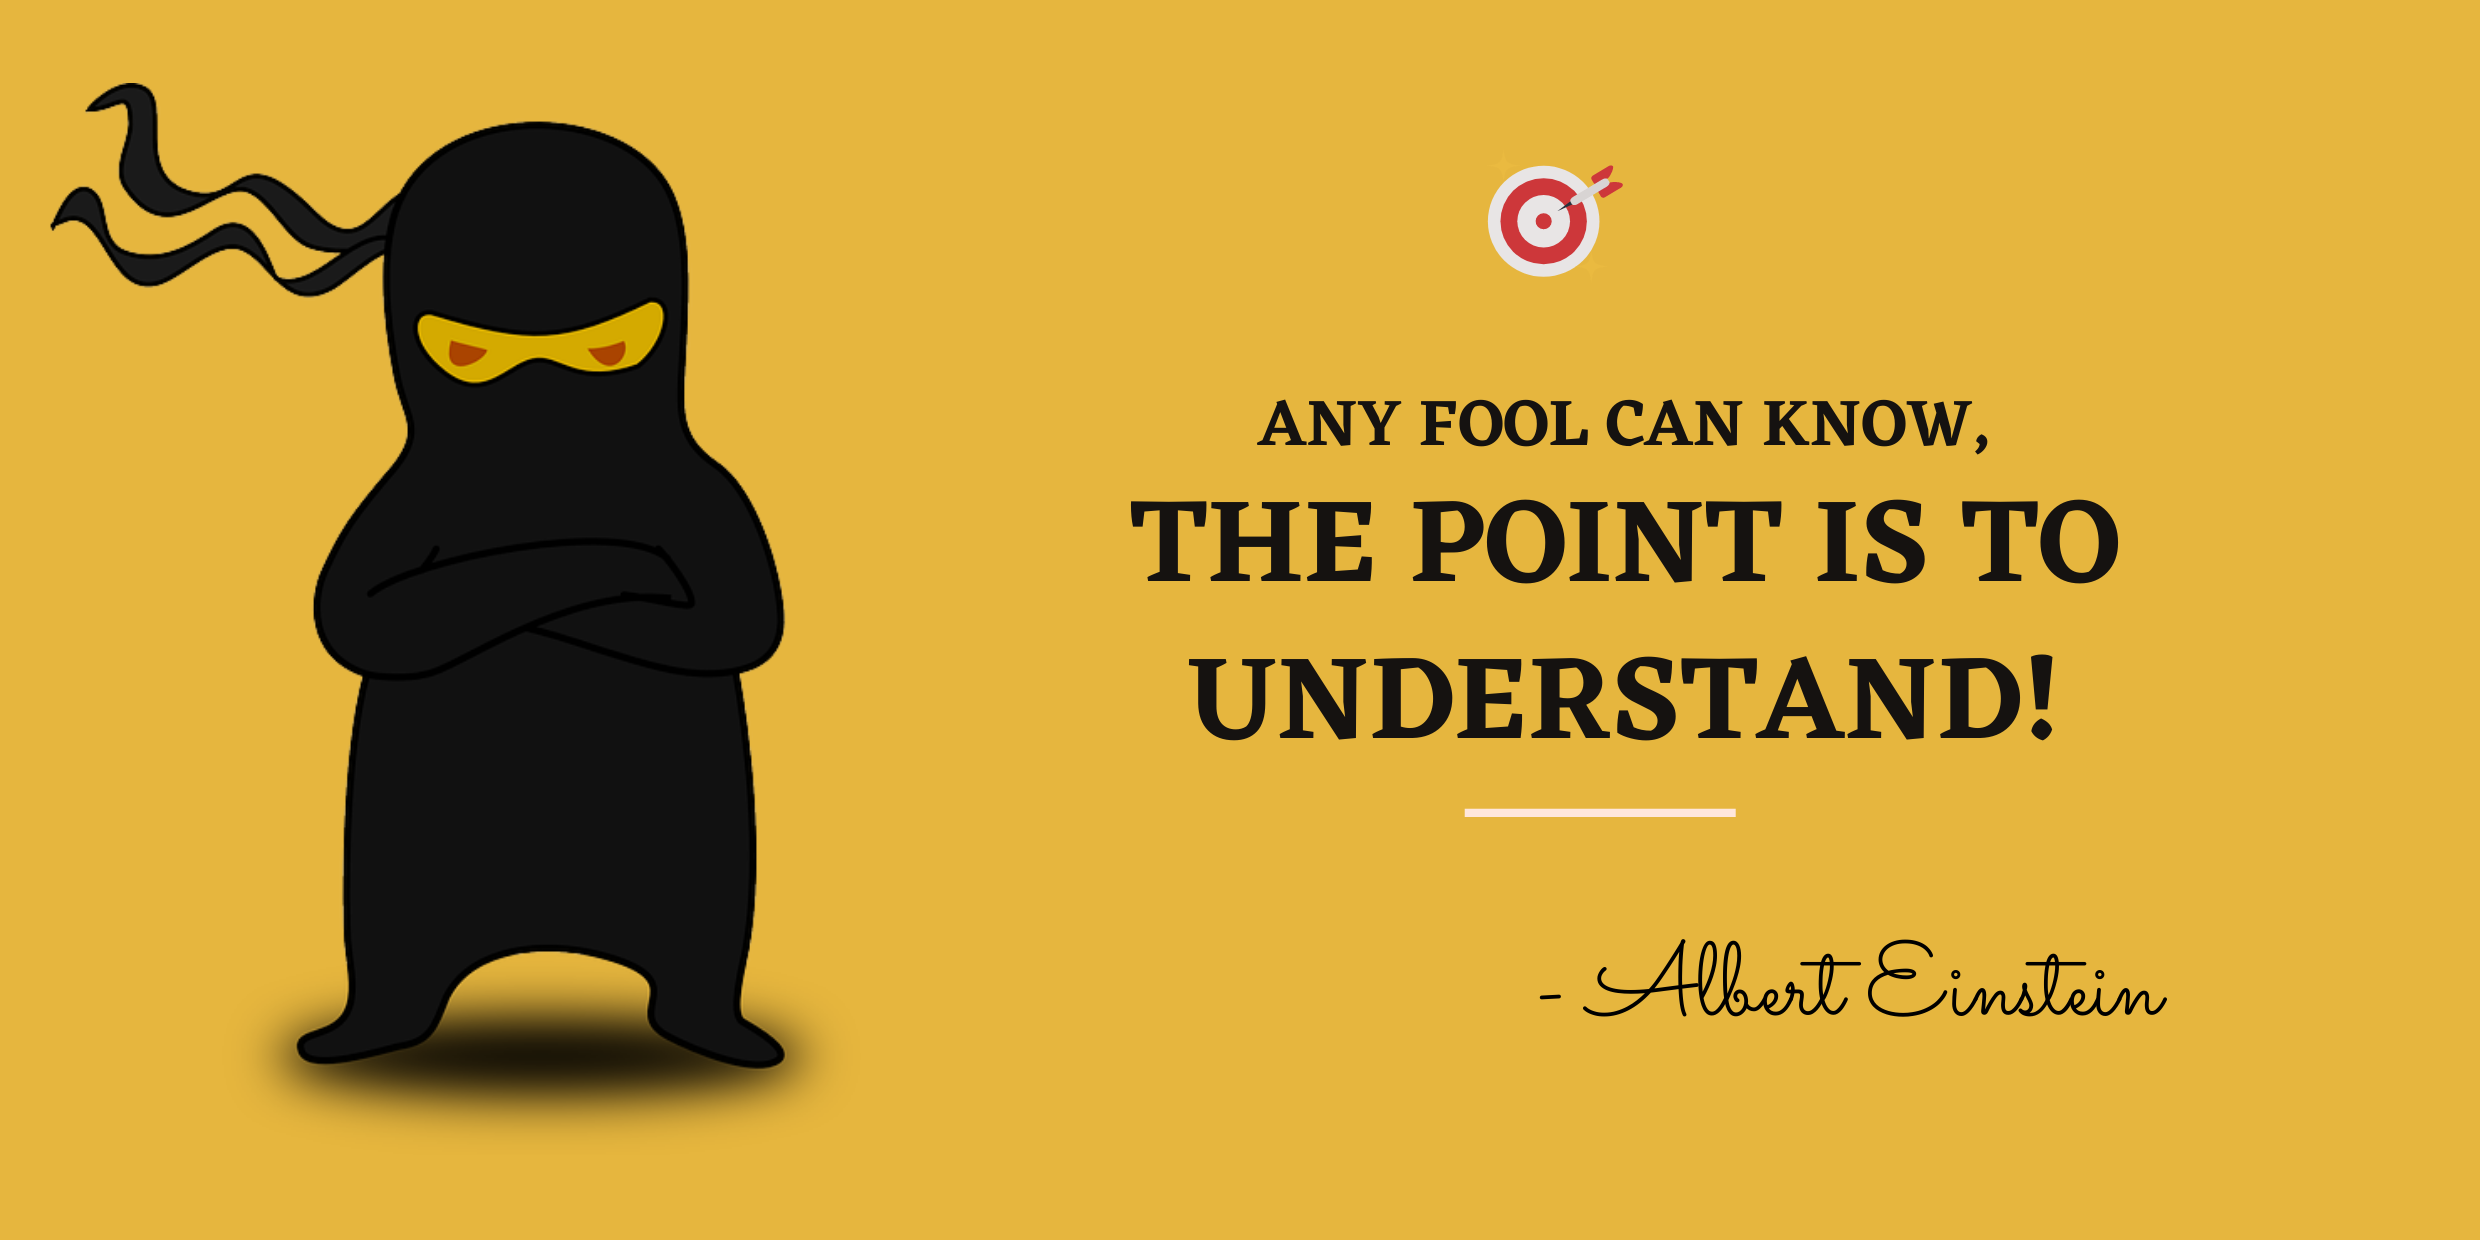
\includegraphics[scale=.2]{content/practise.jpg}
	\end{figure}	
	\begin{enumerate}
		
		\item \textbf{Which of the following is true about RAM? (Select all that applies.)}
		\begin{enumerate}[label=(\alph*)]
			\item RAM stands for Random Access Memory.  %correct
			\item RAM is a computer's short-term memory, which it uses to handle all active tasks and apps. %correct
			\item RAM is used to save file content permanently.
			\item RAM is used to perform arithmetic \& logical processing.
		\end{enumerate}
		\bigskip
		\bigskip
		
		\item \textbf{Which of the following is CPU memory?}
		\begin{enumerate}[label=(\alph*)]
			\item RAM  
			\item Buffer 
			\item Memory cache %correct
			\item Disk cache
		\end{enumerate}
		\bigskip
		\bigskip	
		
		\item \textbf{Which of the following operations uses a buffer? (Select all that applies.)}
		\begin{enumerate}[label=(\alph*)]
			\item Copying data from one device to another where both the device have different data transfer speed. %correct
			\item Print operation. %correct
			\item Holding frequently access data from HDD.
			\item Writing data into a file \& saving it to HDD. %correct
		\end{enumerate}
		\bigskip
		\bigskip	


		\item \textbf{Which of the following command is used to display physical \& swap memory?}
		\begin{enumerate}[label=(\alph*)]
			\item vmstat  
			\item free    %correct
			\item fdisk
			\item netstat
		\end{enumerate}
		\bigskip
		\bigskip	
		
		
		\item \textbf{Which of the following file contains memory details?}
		\begin{enumerate}[label=(\alph*)]
			\item /proc/cpuinfo  
			\item /proc/meminfo         %correct
			\item /etc/fstab
			\item /proc/pid
		\end{enumerate}
		\bigskip
		\bigskip	


		\item \textbf{Which of the following are the warning signs of low memory situations?}
		\begin{enumerate}[label=(\alph*)]
			\item Swap usage is increasing or fluctuating frequently. %correct
			\item Available memory is nearing 0.      %correct
			\item Used memory is close to total memory.
			\item Free memory is close to 0.
		\end{enumerate}
		
	\end{enumerate}
	
	
\end{flushleft}

